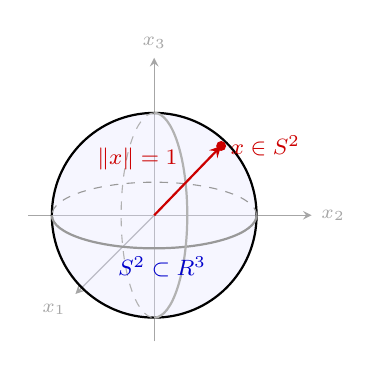
\begin{tikzpicture}[scale=1.0, >=stealth]
  % 3D axes
  \draw[->, gray!70] (-1.6, 0) -- (2.0, 0) node[right, font=\scriptsize] {$x_2$};
  \draw[->, gray!70] (0, -1.6) -- (0, 2.0) node[above, font=\scriptsize] {$x_3$};
  \draw[->, gray!70] (0,0) -- (-1.0, -1.0) node[below left, font=\scriptsize] {$x_1$};
  
  % Sphere
  \draw[thick, fill=blue!10, fill opacity=0.35] (0,0) circle (1.3);
  % Equator
  \draw[dashed, gray!80] (1.3,0) arc (0:180:1.3 and 0.42);
  \draw[thick, gray!80] (-1.3,0) arc (180:360:1.3 and 0.42);
  % Meridian
  \draw[dashed, gray!60] (0,1.3) arc (90:270:0.42 and 1.3);
  \draw[thick, gray!60] (0,1.3) arc (90:-90:0.42 and 1.3);
  
  % Point x on sphere and radius vector
  \draw[->, thick, red!80!black] (0,0) -- (0.85, 0.88) node[midway, above left, font=\footnotesize] {$\|x\|=1$};
  \fill[red!80!black] (0.85, 0.88) circle (1.8pt) node[right, font=\footnotesize] {$x \in S^2$};
  \node[font=\footnotesize, text=blue!80!black] at (0.1, -0.65) {$S^2 \subset \mathbb{R}^3$};
\end{tikzpicture}
